% Source of the figure hardness-construction.pdf: the graph of the reduction from satisfiability for
% phi = (x_1 or not x_2) and (x_2) with 25 vertices: the cliques K^u (top) and K^v (bottom), the rungs u_i v_i,
% the occurrence vertices o_{1,1}, o_{1,2}, o_{2,1} with their edges, and the synchronization edge o_{1,2} o_{2,1}
% (dotted). The clique edges are not drawn. The red path lies in the minimum cut of the assignment x_1 = x_2 = true;
% the dashed curve encloses the side A_tau. Compile with pdfLaTeX; the PDF is included in the manuscript at its
% natural size.
\documentclass[tikz,border=1pt]{standalone}
\usepackage[T1]{fontenc}
\pdfinfoomitdate=1 \pdftrailerid{} \pdfsuppressptexinfo=-1
\definecolor{pathred}{RGB}{200,40,40}
\tikzset{
  vertex/.style={circle, fill=black, inner sep=0pt, minimum size=2.2mm},
  terminal/.style={circle, fill=black, inner sep=0pt, minimum size=3mm},
  occ/.style={circle, draw=black, fill=white, line width=0.9pt, inner sep=0pt, minimum size=3.2mm},
  edge/.style={line width=0.7pt},
  longedge/.style={line width=0.5pt, gray!70},
  syncedge/.style={line width=1pt, dotted, line cap=round},
  pathedge/.style={line width=1.8pt, pathred, line cap=round},
  clique/.style={rounded corners=6pt, fill=gray!14, draw=gray!75!black, line width=0.9pt},
  side/.style={rounded corners=10pt, line width=0.6pt, dash pattern=on 4pt off 3pt, draw=black!70}}
\begin{document}
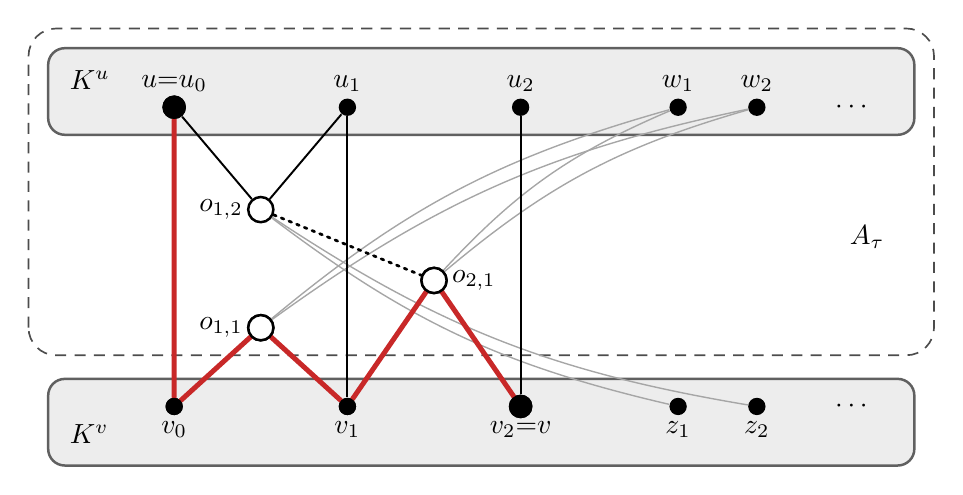
\begin{tikzpicture}[x=1cm, y=1cm]
  \def\yu{4.55}  % row of the vertices of K^u
  \def\yv{0.75}  % row of the vertices of K^v
  % the side A_tau: K^u and the three occurrence vertices
  \draw[side] (-0.25,1.4) rectangle (11.25,5.55);
  \node at (10.4,2.9) {$A_\tau$};
  % the cliques
  \draw[clique] (0,4.2) rectangle (11,5.3);
  \draw[clique] (0,0) rectangle (11,1.1);
  \node[anchor=west] at (0.15,4.9)  {$K^u$};
  \node[anchor=west] at (0.15,0.4)  {$K^v$};
  % vertices of the cliques
  \node[terminal] (u0) at (1.6,\yu) {};
  \node[vertex]   (u1) at (3.8,\yu) {};
  \node[vertex]   (u2) at (6.0,\yu) {};
  \node[vertex]   (w1) at (8.0,\yu) {};
  \node[vertex]   (w2) at (9.0,\yu) {};
  \node[vertex]   (v0) at (1.6,\yv) {};
  \node[vertex]   (v1) at (3.8,\yv) {};
  \node[terminal] (v2) at (6.0,\yv) {};
  \node[vertex]   (z1) at (8.0,\yv) {};
  \node[vertex]   (z2) at (9.0,\yv) {};
  \node at (10.2,\yu) {$\cdots$};
  \node at (10.2,\yv) {$\cdots$};
  \node[above=2pt] at (u0) {$u{=}u_0$};
  \node[above=2pt] at (u1) {$u_1$};
  \node[above=2pt] at (u2) {$u_2$};
  \node[above=2pt] at (w1) {$w_1$};
  \node[above=2pt] at (w2) {$w_2$};
  \node[below=2pt] at (v0) {$v_0$};
  \node[below=2pt] at (v1) {$v_1$};
  \node[below=2pt] at (v2) {$v_2{=}v$};
  \node[below=2pt] at (z1) {$z_1$};
  \node[below=2pt] at (z2) {$z_2$};
  % occurrence vertices
  \node[occ] (o11) at (2.7,1.75) {};
  \node[occ] (o12) at (2.7,3.25) {};
  \node[occ] (o21) at (4.9,2.35) {};
  \node[left=3pt]  at (o11) {$o_{1,1}$};
  \node[left=3pt]  at (o12) {$o_{1,2}$};
  \node[right=3pt] at (o21) {$o_{2,1}$};
  % edges from the occurrence vertices to the anchors
  \draw[longedge] (o11) to[bend left=12] (w1);
  \draw[longedge] (o11) to[bend left=12] (w2);
  \draw[longedge] (o21) to[bend left=12] (w1);
  \draw[longedge] (o21) to[bend left=12] (w2);
  \draw[longedge] (o12) to[bend right=12] (z1);
  \draw[longedge] (o12) to[bend right=12] (z2);
  % short edges, rungs and the synchronization edge
  \draw[edge] (o12) -- (u0) (o12) -- (u1);
  \draw[edge] (u1) -- (v1) (u2) -- (v2);
  \draw[syncedge] (o12) -- (o21);
  % the path in the minimum cut
  \draw[pathedge] (u0) -- (v0) -- (o11) -- (v1) -- (o21) -- (v2);
  % redraw the vertices on the path above the edges
  \foreach \p/\s in {u0/terminal, v0/vertex, v1/vertex, v2/terminal} \node[\s] at (\p) {};
  \foreach \p in {o11, o21} \node[occ] at (\p) {};
\end{tikzpicture}
\end{document}
